\documentclass[final,hyperref={pdfpagelabels=false}]{beamer}
\usepackage{grffile}
\mode<presentation>{\usetheme{I6pd2}}
\usepackage[english]{babel}
\usepackage[latin1]{inputenc}
\usepackage{amsmath,amsthm, amssymb, latexsym}
%\usepackage{times}\usefonttheme{professionalfonts}  % obsolete
%\usefonttheme[onlymath]{serif}
\boldmath
%\usepackage[orientation=portrait,size=a0,scale=1.4,debug]{beamerposter}
\usepackage[size=custom,width=121,height=91,scale=2,debug]{beamerposter}
% change list indention level
% \setdefaultleftmargin{3em}{}{}{}{}{}


%\usepackage{snapshot} % will write a .dep file with all dependencies, allows for easy bundling

\usepackage{array,booktabs,tabularx}
\newcolumntype{Z}{>{\centering\arraybackslash}X} % centered tabularx columns
\newcommand{\pphantom}{\textcolor{ta3aluminium}} % phantom introduces a vertical space in p formatted table columns??!!
\listfiles

\newcommand{\inv}{^{-1}}
\newcommand{\e}{\varepsilon}
\newcommand{\E}{\mathbb{E}}
\newcommand{\N}{\mathbb{N}}
\renewcommand{\P}{\mathbb{P}}
\newcommand{\R}{\mathbb{R}}
\newcommand{\X}{\mathcal{X}}
\newcommand{\Y}{\mathcal{Y}}
\newcommand{\Z}{\mathcal{Z}}
\newcommand{\dist}{\operatorname{dist}}
\newcommand{\vi}{{\vec i}}

%%%%%%%%%%%%%%%%%%%%%%%%%%%%%%%%%%%%%%%%%%%%%%%%%%%%%%%%%%%%%%%%%%%%%%%%%%%%%%%%%%%%%%
\graphicspath{{figures/}}
 
\title{\Large Exponential Concentration of a Density Functional Estimator}
\author{Shashank Singh and Barnab\'as P\'oczos}
\institute[Carnegie Mellon University]{Machine Learning Department,
                            Carnegie Mellon University, Pittsburgh, PA, USA}
\date[December 10, 2014]{December 10, 2014}

%%%%%%%%%%%%%%%%%%%%%%%%%%%%%%%%%%%%%%%%%%%%%%%%%%%%%%%%%%%%%%%%%%%%%%%%%%%%%%%%%%%%%%
\newlength{\columnheight}
\setlength{\columnheight}{75cm}


%%%%%%%%%%%%%%%%%%%%%%%%%%%%%%%%%%%%%%%%%%%%%%%%%%%%%%%%%%%%%%%%%%%%%%%%%%%%%%%%%%%%%%
\begin{document}
\begin{frame}
  \begin{columns}
    % ---------------------------------------------------------%
    % Set up a column 
    \begin{column}{.32\textwidth}
      \begin{beamercolorbox}[center,wd=\textwidth]{postercolumn}
        \begin{minipage}[T]{.95\textwidth}  % tweaks the width, makes a new \textwidth
          \parbox[t][\columnheight]{\textwidth}{ % must be some better way to set the the height, width and textwidth simultaneously
            % Since all columns are the same length, it is all nice and tidy.  You have to get the height empirically
            % ---------------------------------------------------------%
            % fill each column with content            
            \vfill
            \begin{block}{Introduction}
              \begin{itemize}
              \item Many important statistical quantites can be written as
                    \[F(p_1,\dots,p_k)
                        = \int_{\X_1 \times \cdots \times X_k} \hspace{-20mm}
                            f(p_1(x_1),\dots,p_k(x_k)) \; d(x_1,\dots,x_k),\]
                    where each $p_i: \X_i \subseteq \R^d \to \R^+$ is a
                    probability density, $f : \R^k \to \R$ is smooth.
              \item Examples of such quantities, which we call
                    \emph{Density Functionals}, are:
                    \begin{itemize}
                    \item Shannon/KL, R\'enyi-$\alpha$, and Tsallis-$\alpha$
                    entropies, mutual informations, and divergences
                    \item $f$-divergences (e.g., Hellinger, Jensen-Shannon,
                    etc.)
                    \item $L_p$ norms and distances
                    \item Conditional versions of the above quantities
                    \end{itemize}
              \item For many of these quantities, few consistent estimators are
                    known, and almost none of these have finite-sample
                    convergence of concentration guarantees.
              \item We propose and study a nonparametric estimator for such
                    quantities, based on plugging in a boundary-corrected
                    kernel density estimate.
%                    \item For a fixed $\alpha \in [0,1) \cup (1,\infty)$, we
%                    are interested in estimating the R\'enyi-$\alpha$
%                    divergence
%                    \[D_\alpha(p\|q)
%                        = \frac{1}{1 - \alpha} \log \int_\X
%                                        p^\alpha(x)q^{1 - \alpha}(x)) \, dx,\]
%                    between two unknown, continuous, nonparametric probability
%                    densities $p$ and $q$ over $\X \subseteq \R^d$, using
%                    samples from each density.
%              \item Applications of divergence estimation include
%                \begin{itemize}
%                \item extending machine learning algorithms designed to operate
%                      on finite-dimensional feature vectors to the setting
%                      where inputs are sets or distributions.
%                \item estimating entropy and mutual information.
%                \end{itemize}
              \item We prove that, when each $\X_i = [0,1]^d$ is a unit cube:
                \begin{itemize}
                \item our estimator is exponentially concentrated about its
                      mean.
                \item for densities in a $\beta$-H\"older smoothness class with
                      certain boundary conditions, the bias of the estimator
                      decays as $O\left(n^{-\frac{\beta}{\beta + d}}\right)$,
                      where $n$ is the number of samples from each density.
                \end{itemize}
              \end{itemize}
            \end{block}
%            \vfill
%            \begin{block}{Problem Statement}
%            {\footnotesize
%            Given a positive integer $d$, consider two probability densities
%            $p,q : \X = [0,1]^d \to \R$ on the unit cube, with known positive
%            lower and upper bounds $\kappa_1,\kappa_2 \in \R$
%            ($0 < \kappa_1 \leq p,q \leq \kappa_2 < \infty$). For a given
%            $\alpha \in [0,1) \cup (1,\infty)$, we are interested in using
%            random samples of $x^1,\dots,x^n \in \X$ and $y^1,\dots,y^n$ of $n$
%            i.i.d. points from $p$ and $q$, respectively, to estimate
%            $D_\alpha(p\|q)$.}
%\begin{enumerate}[]
%\item
%\end{enumerate}
%\vspace{-10mm}
%            \end{block}
            \vfill
            \begin{block}{Assumptions}
              {\footnotesize
              Let $\beta > 0$, and let $\ell := \lfloor \beta \rfloor$ be
              the greatest integer \emph{strictly} less than $\beta$. We make
              the following four assumptions on $f$, the densities
              $p_1,\dots,p_k$, the kernel $K$:\\}
              \begin{itemize}
              \item {\bf\footnotesize ($f$-Smoothness)} $f$ is twice
              continuously differentiable.
              \item {\bf\footnotesize (Density Smoothness)} All (mixed)
              $\ell$-order partial derivatives of $p_1,\dots,p_k$ exist and are
              $(\beta - \ell)$-H\"older Continuous (i.e., there exists
              $L \in \R$ such that, $\forall x, x + v \in \X$, $|\vi| = \ell$,
              each
                    \[|D^\vi p_i(x + v) - D^\vi p_i(x)|
                                        \leq L\|v\|_2^{\beta - \ell}\mbox{)}.\]
              \item {\bf\footnotesize (Density Boundaries)} All derivatives of
                    $p_1,\dots,p_k$ of order up to $\ell$ vanish at the boundary
                    \[\partial\X = \{x \in \X : x_i \in \{0,1\}
                                            \mbox{ for some } i \in [d]\}\]
                    (i.e., $\sup_{1 \leq |\vi| \leq \ell} |D^\vi(x)| \to 0$
                    as $\dist(x,\partial\X) \to 0$).
                    \vspace{1cm}
              \item {\bf\footnotesize (Kernel)} The kernel
                    $K : \R \to \R$ has support in $[-1,1]$,
                    \[\hspace{-15mm}\int_{-1}^1 K(u) \, du = 1
                                    \quad \mbox{ and } \quad
                                    \int_{-1}^1 u^j K(u) \, du = 0,
                                    \quad
                                    \forall j \in \{1,\dots,\ell\}.\]
              \end{itemize}
            \end{block}
            \vfill
          }
        \end{minipage}
      \end{beamercolorbox}
    \end{column}
    % ---------------------------------------------------------%
    % end the column

    % ---------------------------------------------------------%
    % Set up a column 
    \begin{column}{.32\textwidth}
      \begin{beamercolorbox}[center,wd=\textwidth]{postercolumn}
        \begin{minipage}[T]{.95\textwidth} % tweaks the width, makes a new \textwidth
          \parbox[t][\columnheight]{\textwidth}{ % must be some better way to set the the height, width and textwidth simultaneously
            % Since all columns are the same length, it is all nice and tidy.  You have to get the height empirically
            % ---------------------------------------------------------%
            % fill each column with content
            \vfill
            \begin{block}{Mirrored Kernel Density Estimator}
              \begin{columns}
                \begin{column}{.63\textwidth}
                  {\footnotesize
                  Given a bandwidth $h$, our density functional estimate is
                  computed in 3 steps:}
                  \vspace{12mm}
                  \begin{enumerate}
                  \item Augment data from $p_i$ with reflections over each
                        subset of edges of $\X_i$.
                  \item Compute kernel density estimates
                        $\hat p_1,\dots,\hat p_k$ from the augmented data,
                        using a product kernel and bandwidth $h$.
                  \item Estimate $F(p_1,\dots,p_k)$ by the plug-in estimator
                        $F(\hat p_1,\dots,\hat p_k)$.
                  \end{enumerate}
                \end{column}
                \begin{column}{.36\textwidth}
                  \begin{figure}[h!]
                    \centering
                    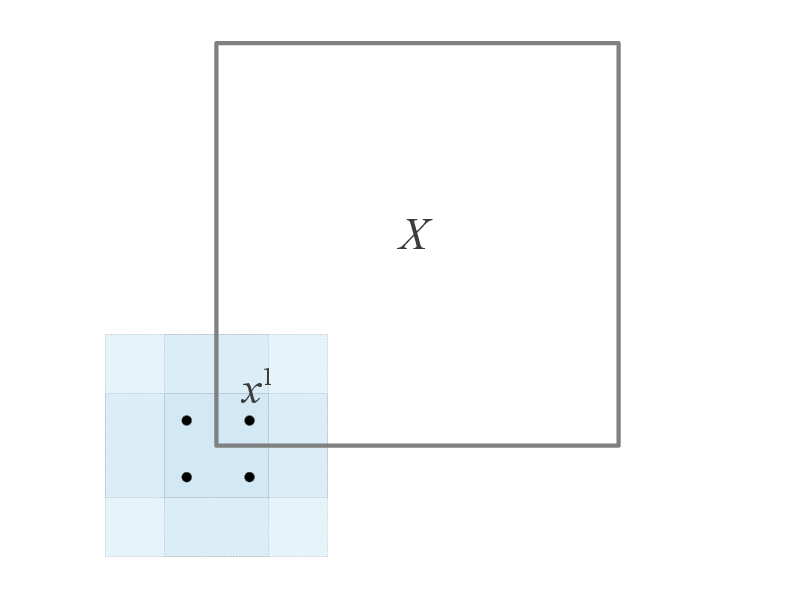
\includegraphics[width=\linewidth]{figures/mirror_fig}
                    \caption{\scriptsize Four kernels centered on a single data
                                         point and its three reflected copies,
                                         in the case $d = 2$.}
                    \label{fig:mirror_fig}
                  \end{figure}
                \end{column}
              \end{columns}
            \end{block}
            \vfill
            \begin{block}{\normalsize Results: Exponential Concentration Bound}
              \begin{itemize}
              \item We show that, $\forall \e > 0$,
                \[\P\left(
                        \left| F(\hat p_1,\dots,\hat p_k)
                           - \E F(\hat p_1,\dots,\hat p_k) \right|
                        > \e
                    \right)
                    \leq 2\exp\left( -\frac{\e^2n}{C_V^2} \right),\]
              where $C_V = 2C_f\|K\|_1^d$ is constant in $n$ and $h$.
              \item Main tool in proof is McDiarmid's Inequality, by which it
              suffices to bound the change in the estimate when resampling a
              single data point by $C_V/n$.
              \item This is achieved by combining the smoothness of $f$ with
                    the observation that the integral of the mirrored kernel
                    density estimate changes by at most
                    $\frac{2}{n} \|K\|_1^d$.
              \end{itemize}
            \end{block}
            \vfill
            \begin{block}{Results: Convergence Rate}
              \begin{itemize}
              \item We show there exists $C_B \in \R$ (constant in $n$ and $h$)
                    such that
                    \[|\E F(\hat p_1,\dots,\hat p_k) - F(p_1,\dots,p_k)|
                    \leq C_B\left( h^\beta + \frac{1}{nh^d} \right).\]
              \item Previous work \cite{singh14exponential} bounded the
                    integral of each mirrored kernel density estimator's
                    pointwise squared bias:
                    \begin{equation}
                    \int_{\X_i} (\E \hat p_i(x) - p(x))^2 \, dx
                                                        \leq C_b h^{2\beta}
                    \label{ineq:bias_lemma}
                    \end{equation}
              \item To derive our convergence rate, we make a second-order
                    Taylor estimate of $f$ and then use H\"older's Inequality
                    to reduce the resulting terms to (\ref{ineq:bias_lemma})
                    and the integrated mean squared error of a standard kernel
                    density estimator.
              \end{itemize}
            \end{block}
            \vfill
          }
        \end{minipage}
      \end{beamercolorbox}
    \end{column}
    % ---------------------------------------------------------%
    % end the column

    % ---------------------------------------------------------%
    % Set up a column 
    \begin{column}{.32\textwidth}
      \begin{beamercolorbox}[center,wd=\textwidth]{postercolumn}
        \begin{minipage}[T]{.95\textwidth} % tweaks the width, makes a new \textwidth
          \parbox[t][\columnheight]{\textwidth}{ % must be some better way to set the the height, width and textwidth simultaneously
            % Since all columns are the same length, it is all nice and tidy.  You have to get the height empirically
            % ---------------------------------------------------------%
            % fill each column with content
            \vfill
            \begin{block}{Condition Density Functionals}
                  \begin{itemize}
                  \item It is often useful to condition density functionals on
                        one or more additional variables; e.g., to estimate
                        \[F(P)
                            = \int_\Z P_Z(z) f\left(
                                    \int_\X g\left(
                                        \frac{P_{X,Z}(x,z)}{P_Z(z)}
                                    \right) \, dx
                                \right) \, dz.\]
                  \item For example, conditional entropy estimation has
                        applications to clustering \cite{steeg2013demystifying}
                        and conditional mutual information is useful for
                        learning graphical models
                        \cite{koller09probgraphmodels}.
                  \item As long as the density of the conditioned variable
                        (e.g., $P_Z$) has a positive lower bound, our results
                        extend to the mirrored kernel density plug-in
                        estimator for such
                        \emph{conditional density functionals}.
                  \end{itemize}
            \end{block}
            \vfill
            \begin{block}{Discussion}
                  \begin{itemize}
                  \item The exponential concentration bound gives a bound on
                        the variance of the estimator:
                        \vspace{-5mm}
                        \[\mathbb{V}[F(\hat p_1,\dots,\hat p_k)]
                                                    \leq C_V^2n\inv.\]
                  \item This does not depend on $h$, so pick $h$ to minimize
                        the bias bound.
                        \begin{itemize}
                        \item Asymptotically, the optimal $h$ is
                              $h \asymp n^{-\frac{1}{\beta + d}}$, so bias
                              bound is
                              $O\left( n^{-\frac{\beta}{\beta + d}} \right)$.
                        \end{itemize}
                  \item Hence MSE is $O(n^{-\frac{2\beta}{\beta + d}}+n\inv)$,
                        which is the parametric rate $O(n\inv)$ if
                        $\beta \geq d$ and $O(n^{-\frac{\beta}{\beta + d}})$
                        otherwise.
                  \item Kernel assumptions for the bias bound necessitate
                        $\|K\|_1 > 1$ when $\beta \geq 2$ and $C_V$ includes
                        $\|K\|_1^d$, which is exponential in $d$.
                        \begin{itemize}
                        \item Lower bounds in $d$ are unknown; whether
                        dependence is necessarily exponential is an important
                        open problem.
                        \end{itemize}
                  \item For divergences and information theoretic density
                        functionals, the integral in the plug-in estimator can
                        be well estimated by a sample mean. In this case, our
                        estimator can be computed in $O(2^d n \log n)$, making
                        it effective for large, low-dimensional datasets.
                  \end{itemize}
            \end{block}
%            \vfill
%            \begin{block}{The R\'enyi-$\alpha$ Divergence and Conditional
%                                                    Mutual Information Cases}
%            Fix $\alpha \in [0,1) \cup (1,\infty)$. Two particular density
%            functionals of interest are R\'enyi-$\alpha$ Divergence
%            \[D_\alpha(p_1\|p_2) = \frac{1}{1 - \alpha} \log
%                        \int_{\X} p_1^\alpha(x)p_2^{1 - \alpha}(x) \, dx,\]
%            where $p_1$ and $p_2$ are densities, and R\'enyi-$\alpha$
%            Conditional Mutual Information
%            \begin{align*}
%            & I_\alpha(X;Y | Z) \\
%            & = \int_\Z \frac{P(z)}{1 - \alpha} \log
%            \int_{\X \times \Y} \left( \frac{P(x,y,z)}{P(z)} \right)^\alpha
%            \left( \frac{P(x,z)P(y,z)}{P^2(z)} \right)^{1 - \alpha}
%            \hspace{-20mm} d(x,y) dz,
%            \end{align*}
%            where $X$, $Y$, and $Z$ are random variables and $P$ denotes their
%            joint density, as well as its marginal densities.
%            \end{block}
            \vfill
            \begin{block}{References}
                {
                \footnotesize
                \bibliographystyle{plain}
                \bibliography{biblio}
                }
            \end{block}
            \vfill
          }
          % ---------------------------------------------------------%
          % end the column
        \end{minipage}
      \end{beamercolorbox}
    \end{column}
    % ---------------------------------------------------------%
    % end the column
  \end{columns}
  \vskip1ex
  %\tiny\hfill\textcolor{ta2gray}{Created with \LaTeX \texttt{beamerposter}  \url{http://www-i6.informatik.rwth-aachen.de/~dreuw/latexbeamerposter.php}}
  {\tiny\hfill\LaTeX \texttt{beamerposter}  \url{http://www-i6.informatik.rwth-aachen.de/~dreuw/latexbeamerposter.php} \hskip1em}
\end{frame}
\end{document}


%%%%%%%%%%%%%%%%%%%%%%%%%%%%%%%%%%%%%%%%%%%%%%%%%%%%%%%%%%%%%%%%%%%%%%%%%%%%%%%%%%%%%%%%%%%%%%%%%%%%
%%% Local Variables: 
%%% mode: latex
%%% TeX-PDF-mode: t
%%% End:
